\section{程序出错之后，从哪里开始？}

\begin{frame}{HW1：完整代码（调试用错误版）}
    \small 依据HW1 P3要求编写的课堂调试变体：读整数至0，输出总和与最大值。
    \lstset{basicstyle=\ttfamily\fontsize{7.5}{8.8}\selectfont,
        numberstyle=\fontsize{4.8}{5.5}\selectfont\color{gray},xleftmargin=6pt}
    \begin{columns}[T]
        \begin{column}{0.48\textwidth}
            \begin{Code}*{c}
                \lstinputlisting[firstline=1,lastline=14,firstnumber=1]{code/homework/hw1-p3.c}
            \end{Code}
        \end{column}
        \begin{column}{0.48\textwidth}
            \begin{Code}*{c}
                \lstinputlisting[firstline=15,firstnumber=15,lastline=30]{code/homework/hw1-p3.c}
            \end{Code}
        \end{column}
    \end{columns}
    \note{完整展示现有HW1错误版，不使用数组或动态内存。先让学生预测程序输出，再用下一页的小输入检验。错误位于更新最大值时传入了sum而不是x；后续用GDB观察调用者和被调用函数中的变量。现场演示直接使用code/homework/hw1-p3.c。}
\end{frame}

\begin{frame}{HW1：编译通过，然后呢？}
    P3的starter要求：读整数，遇到0结束，输出\alert{总和与最大值}；不用数组或动态内存。
    \begin{columns}[T]
        \begin{column}{0.52\textwidth}
            \begin{block}{课堂运行截图}
                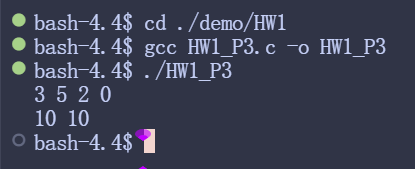
\includegraphics[width=\linewidth,height=0.42\textheight,keepaspectratio]{HW1_P3.png}
            \end{block}
            输入：\texttt{3 5 2 0}。\par
            0是结束标记，不是待统计的数据。
        \end{column}
        \begin{column}{0.44\textwidth}
            \begin{itemize}
                \item 总和：$3+5+2=10$。
                \item 最大值：5。
                \item 预期输出：\texttt{10 5}。
                \item 错误版输出：\alert{\texttt{10 10}}。
            \end{itemize}
        \end{column}
    \end{columns}
    \medskip
    \alert{能编译、能运行，不代表实现了需求。}先用小输入找出差异。
    \note{截图使用用户提供的image/HW1_P3.png，展示编译成功后输入3 5 2 0却输出10 10的现象。先对照手算结果，再进入后续调试流程。}
\end{frame}

\begin{frame}{先说清楚：错在哪里？}
    \begin{center}
        \renewcommand{\arraystretch}{1.4}
        \begin{tabular}{p{0.23\linewidth}p{0.60\linewidth}}
            \textbf{现象} & \textbf{第一步要收集什么？} \\
            编译或链接失败 & 完整命令、第一条诊断、对应源码。 \\
            运行崩溃 & 能复现的输入、信号、调用栈。 \\
            输出错误 & 明确的预期结果、一个小反例。 \\
            一直不结束 & 输入是否读完、程序停在哪个循环或调用。
        \end{tabular}
    \end{center}
    \medskip
    “我的程序有问题”还不够。先补全：\alert{输入是什么？应该怎样？实际怎样？}
\end{frame}

\begin{frame}{一次只验证一个猜想}
    对于输出\texttt{10 10}的HW1课堂变体，先问：
    \begin{enumerate}
        \item 是否依次读到了3、5、2，并在0处停止？
        \item 每轮结束后，总和是否依次为3、8、10？
        \item 最大值是否依次为3、5、5？
        \item 传给更新最大值函数的，是当前输入，还是别的量？
    \end{enumerate}
    \medskip
    \begin{vspquotered}{让猜想可以被验证}
        写下“这里应该是多少”，再观察“这里实际是多少”。\par
        保留失败输入，每次修改后重新运行。
    \end{vspquotered}
\end{frame}

\begin{frame}{从复现到验证：工具分别帮什么忙？}
    \begin{center}
        \begin{tikzpicture}[node distance=0.27cm,>=Stealth,
            every node/.style={font=\small},
            stage/.style={draw=VSPPrimary,rounded corners,align=center,
                minimum width=1.85cm,minimum height=0.8cm}]
            \node[stage] (a) {复现错误};
            \node[stage,right=of a] (b) {缩小范围};
            \node[stage,right=of b] (c) {观察状态};
            \node[stage,right=of c] (d) {解释原因};
            \node[stage,right=of d] (e) {修复验证};
            \draw[->] (a)--(b); \draw[->] (b)--(c);
            \draw[->] (c)--(d); \draw[->] (d)--(e);
        \end{tikzpicture}
    \end{center}
    \begin{itemize}
        \item \alert{编译警告}：编译时发现可疑写法；逐条阅读。
        \item \alert{日志与断言}：记录关键状态，检查必须成立的条件。
        \item \alert{GDB}：观察变量、执行位置与调用栈。
        \item \alert{Sanitizer}：在运行时检查特定类别的非法行为。
    \end{itemize}
    工具提供线索；预期结果与原因解释，需要你来确定。
    \note{本节约8分钟。先让学生手算总和10与最大值5，再预测每轮的中间状态。}
\end{frame}
